%----------------------------------------------------------------
%
%  File    :  chapter6.tex
%
%  Authors : Michael Fuska, FH Campus Wien, Austria% 
%  Created : 13 Feb 2016
%
%  Changed :  
% 
%----------------------------------------------------------------


\chapter{Analyse und Ergebnisse}
\label{ch:Ergebnisse}

%------------------------------------------------------------------------------
%------------------------------ Encryption and Data Protection
\section{Frage 1}
\label{sec:Frage1}

\begin{description}
    \item[\parbox{\textwidth} {Antwort kurz INFO Katharina}]~\par
    \begin{itemize}
          \item iOS HW (Tabelle \ref{tab:iOSHW})
           \item iOS SW (Tabelle \ref{tab:iOSVersion})
           \item JB  (Abbildung: \ref{fig:AnalyseiOSJB1},Abbildung: \ref{fig:AnalyseiOSJB2})
    \end{itemize}
\end{description} 

\begin{table}[htp!]
    \begin{center}
        \begin{tabular}{|l|l|l|l|l|l|} \hline
            \textbf{iOS Device} & \textbf{Verkaufsstart} & \textbf{Tage JB} & \textbf{initial iOS} & \textbf{last iOS }& \textbf{Prozessor}\\ \hline
            iPhone & 29.06.2007 & 11 & 1.0 & 3.1.3 & Samsung SSL8900\\ \hline
            iPhone 3G & 11.07.2008 & 9 & 2.0 & 4.2.1 & Samsung SSL8900 \\ \hline
            iPhone 3GS & 19.06.2009 & 14 & 3.0 & 6.1.6 & Samsung SSL 8920 \\ \hline
            iPhone 4 & 01.08.2010 & 38 & 4.0 & 7.1.2 & Apple A4 \\ \hline
            iPhone 4s & 20.01.2012 & 98 & 5.0 & 9.3.2 & Apple A5 \\ \hline 
            iPhone 5 & 21.09.2012 & 136 & 6.0 & 9.3.2 & Apple A6 \\ \hline
            iPhone 5c & 22.12.2013 & 93 & 7.0 & 9.3.2 & Apple A6 \\ \hline
            iPhone 5s & 22.12.2013 & 93 & 7.0 & 9.3.2 & Apple A7 \\ \hline
            iPhone 6 & 19.09.2014 & 33 & 8.0 & 9.3.2 & Apple A8 \\ \hline
            iPhone 6 Plus & 19.09.2014 & 33 & 8.0 & 9.3.2 & Apple A8 \\ \hline
            iPhone 6s & 25.09.2016 & 19 & 9.0 & 9.3.2 & Apple A9 \\ \hline
            iPhone 6s Plus & 25.09.2016 & 19 & 9.0 & 9.3.2 & Apple A9 \\ \hline
            iPhone SE & 31.03.2016 & nA & 9.0 & 9.3.2 & Apple A9 \\ \hline  
        \end{tabular} 
        \caption{Sicherheitszusammenhang iOS Device und JB }
        \label{tab:iOSHW}
    \end{center}
\end{table}

\begin{table}[htp!]
    \begin{center}
        \begin{tabular}{|l|l|l|} \hline
         \textbf{iOS Version} & \textbf{Veröffentilicht} & \textbf{Tage JB}\\ \hline    
        1.0 & 29.06.2007 & 11\\ \hline 
        2.0 & 11.07.2008	& 9\\ \hline 
        3.0 & 17.06.2009	& 2\\ \hline 
        4.0 & 21.06.2010 & 2\\ \hline 
        5.0 & 12.10.2011	& 1\\ \hline 
        6.0 & 19.09.2012	& 0\\ \hline 
        7.0 & 18.09.2013	& 95\\ \hline 
        7.1-7.1.2 & 29.05.2014 & 25\\ \hline 
        8.0 & 17.09.2014	& 35\\ \hline 
        8.1.1-8.4 & 17.11.2014	& 12\\ \hline 
        9.0 & 16.09.2015	& 28\\ \hline 
        9.1 & 21.10.2015	& 142\\ \hline 
        \end{tabular} 
        \caption{Sicherheitszusammenhang iOS Version und JB}
        \label{tab:iOSVersion}
    \end{center}
\end{table}
         
\begin{figure}[htbp]
        \centering
                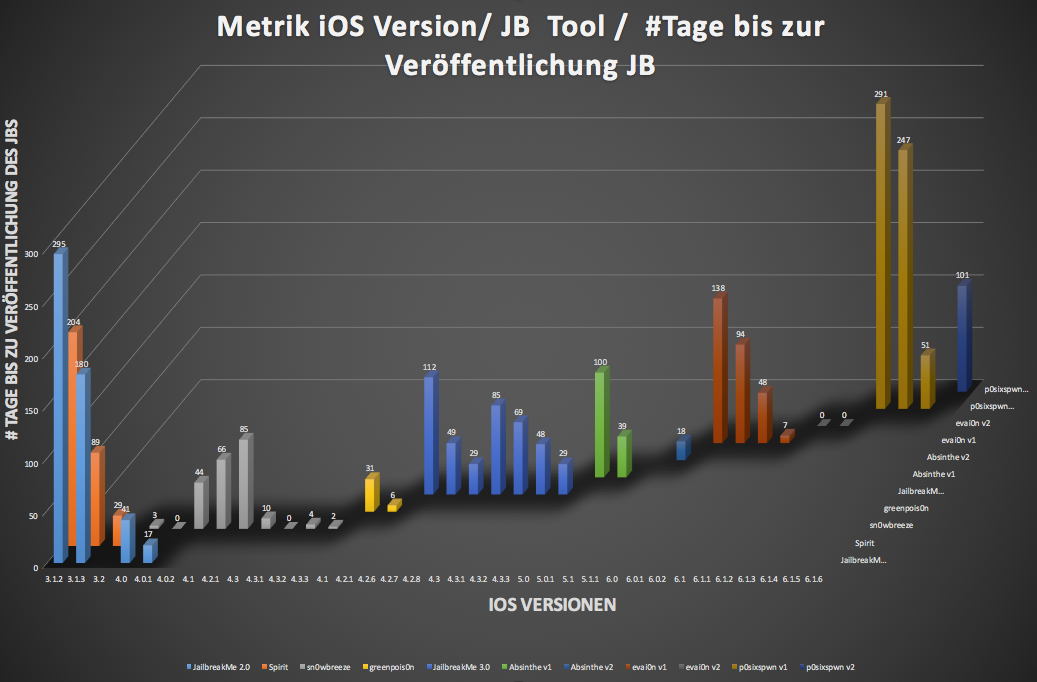
\includegraphics[height=11cm]{Bilder/Frage1_1.png}
        \caption{iOS Version / JB / Tage}
        \label{fig:AnalyseiOSJB1}        
\end{figure}

\begin{figure}[htbp]
        \centering
                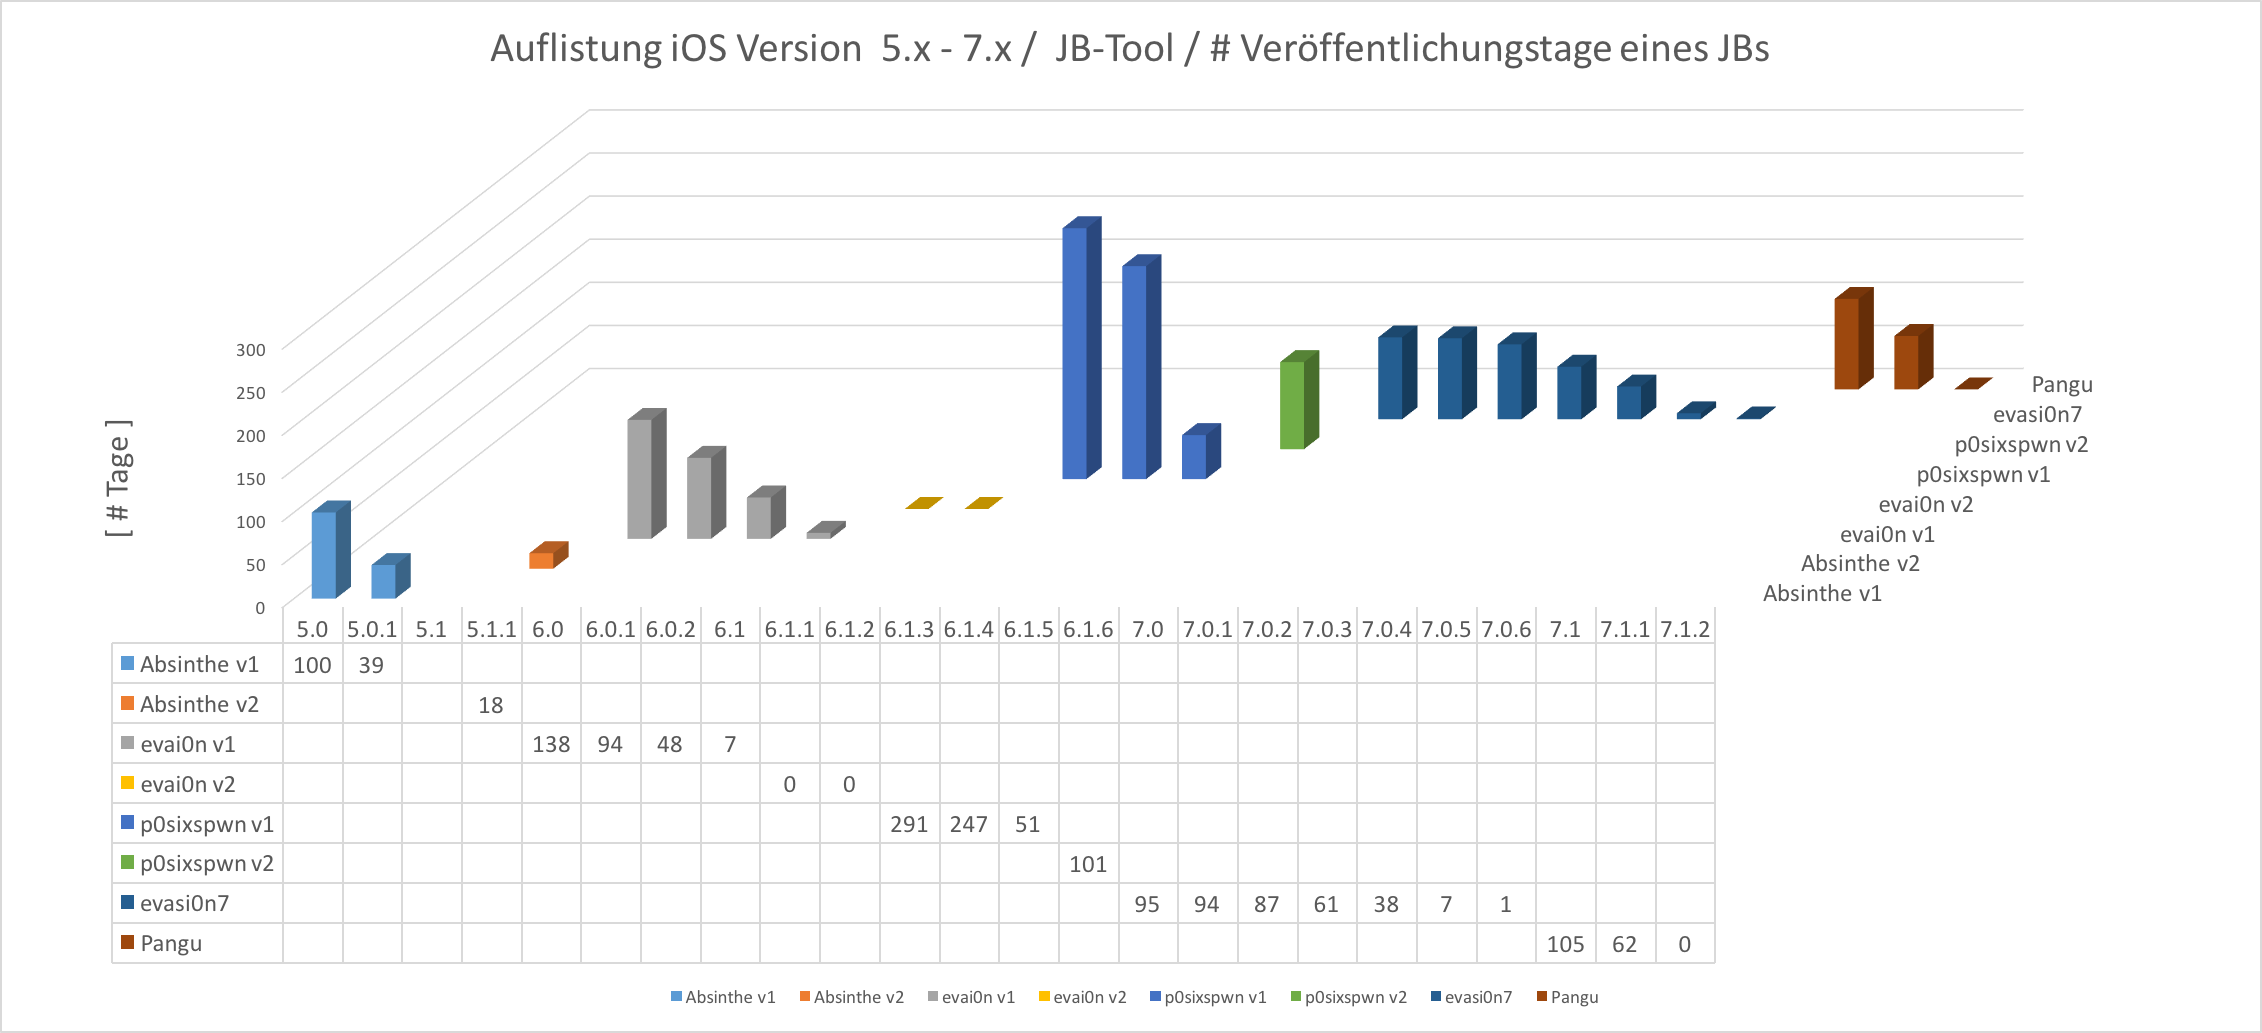
\includegraphics[height=10cm]{Bilder/Frage1_2.png}
        \caption{iOS Version / JB / Tage}
        \label{fig:AnalyseiOSJB2}
\end{figure}

\section{Frage 2}
\label{sec:Frage2}

\begin{description}
    \item[\parbox{\textwidth} {Antwort kurz INFO Katharina}]~\par
        \begin{itemize}
                \item Zuordnung Bugs / Sicherheitsmechanismen Ausreißer in den Stats Veröffentlichung \#Tage JB  
        \end{itemize}
\end{description} 
        


\section{Frage 3}
\label{sec:Frage3}

\begin{description}
    \item[\parbox{\textwidth} {Antwort kurz INFO Katharina}]~\par
        \begin{itemize}
                \item \#Tage Gültigkeit eines JB -> Erklärung Dauer / Ausreißer
                \item \#Geschlossene Bugs (Apple / JB)   -> Erklärung 
        \end{itemize}
\end{description} 
 